% \iffalse
\let\negmedspace\undefined
\let\negthickspace\undefined
\documentclass[journal,12pt,twocolumn]{IEEEtran}
\usepackage{cite}
\usepackage{amsmath,amssymb,amsfonts,amsthm}
\usepackage{algorithmic}
\usepackage{graphicx}
\usepackage{textcomp}
\usepackage{xcolor}
\usepackage{txfonts}
\usepackage{listings}
\usepackage{enumitem}
\usepackage{mathtools}
\usepackage{gensymb}
\usepackage{comment}
\usepackage[breaklinks=true]{hyperref}
\usepackage{tkz-euclide}
\usepackage{listings}
\usepackage{gvv}
\def\inputGnumericTable{}
\usepackage[latin1]{inputenc}
\usepackage{color}
\usepackage{array}
\usepackage{longtable}
\usepackage{calc}
\usepackage{multirow}
\usepackage{hhline}
\usepackage{ifthen}
\usepackage{lscape}

\newtheorem{theorem}{Theorem}[section]
\newtheorem{problem}{Problem}
\newtheorem{proposition}{Proposition}[section]
\newtheorem{lemma}{Lemma}[section]
\newtheorem{corollary}[theorem]{Corollary}
\newtheorem{example}{Example}[section]
\newtheorem{definition}[problem]{Definition}
\newcommand{\BEQA}{\begin{eqnarray}}
\newcommand{\EEQA}{\end{eqnarray}}
\newcommand{\define}{\stackrel{\triangle}{=}}
\theoremstyle{remark}
\newtheorem{rem}{Remark}
\begin{document}

\bibliographystyle{IEEEtran}
\vspace{3cm}

\title{GATE 2022  -AE 63}
\author{EE23BTECH11057 - Shakunaveti Sai Sri Ram Varun$^{}$% &lt;-this % stops a space
}
\maketitle
\newpage
\bigskip
\vspace{2cm}
\textbf{Question: }
A two degree of freedom spring-mass system undergoing free vibration
with generalized coordinates $ x_1$ and $ x_2$ has natural frequencies $ \omega_1=233.9\text{ rad/s}$ and $ \omega_2 = 324.5\text{ rad/s}$ , respectively. The corresponding mode shapes $ \phi_1=\begin{bmatrix}
1\\
-3.16
\end{bmatrix}$ and $ \phi_2=\begin{bmatrix}
1\\
3.16\end{bmatrix}$. If the system is disturbed with certain
deflections and zero initial velocities, then which of the following
statement(s) is/are true?


\begin{enumerate}
    \item[(A)] An initial deflection of $ x_1\brak{0}=6.32$cm and $ x_2\brak{0}=-3.16$cm would make the system oscillate with only the second natural frequency.
    \item[(B)]An initial deflection of $ x_1\brak{0}=2$cm and $ x_2\brak{0}=-6.32$cm would make the system oscillate with only the first natural frequency.
    \item[(C)] An initial deflection of $ x_1\brak{0}=2$cm and $ x_2\brak{0}=-2$cm would make the system oscillate with linear combination of first and second natural frequency.
    \item[(D)] An initial deflection of $ x_1\brak{0}=1$cm and $ x_2\brak{0}=-6.32$cm would make the system oscillate with only the first natural frequency.
\end{enumerate}
\hfill(GATE AE 2021 QUESTION 32)\\
\textbf{Solution}:\\
\begin{table}[h!] 
\centering
\begin{tabular}{|c|c|c|}
    \hline
    \textbf{Parameter} & \textbf{Description} & \textbf{Value} \\
    \hline
    $X\brak{s}$ & position in laplace domain & $ X\brak{s}$ \\
    \hline
    $\Theta\brak{s}$ & angle rotated in laplace domain & $ \Theta\brak{s}$ \\
    \hline
    $x\brak{t}$ & position of mass w.r.t time & $x\brak{t}$ \\
    \hline
    $\theta\brak{t}$ & angle rotated by mass w.r.t time &$ \theta\brak{t}$\\
    \hline
    $\alpha\brak{t}$ & angular acceleration of mass w.r.t time & $\alpha\brak{t}$ \\
    \hline
    $k$ & spring constant & $ k$\\
    \hline
    $m$ & mass of the block & $ m$\\
    \hline
    $L$ & length of the mass & $ L$\\
    \hline
    $\omega_o$ & initial angular velocity of mass & $ \omega_o$ \\
    \hline
    $v\brak{0}$ & initial velocity of mass& $ v\brak{0}$ \\
    \hline
    
\end{tabular}






\caption{input values}
\label{tab: Table2021_ae_32_1}
\end{table}
\begin{figure}[h!]
    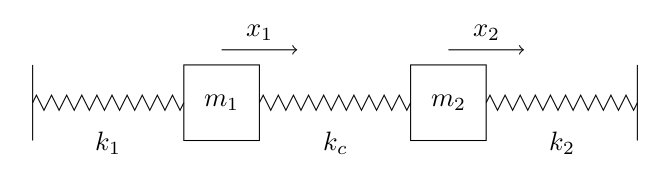
\includegraphics[width = \columnwidth]{figs/qn_fig.png}
    \caption{System with D.O.F =2}
    \centering
    \label{fig: ae_32_`1_fig}
\end{figure}

The F.B.D for above system is written as:
\begin{align}
m_1 \frac{d^2 x_1}{dt^2} - k_c\brak{x_2-x_1} + k_1 x_1 &=0\\
m_2 \frac{d^2 x_2}{dt^2} + k_c\brak{x_2-x_1} + k_2 x_2 &=0
\end{align}
Which can be written in the form of matrices as:
\begin{align}
\begin{bmatrix}
m_1&0\\
0&m_2\end{bmatrix}
\begin{pmatrix}
\frac{d^2x_1}{dt^2}\\
\frac{d^2x_2}{dt^2}
\end{pmatrix}
&= -\begin{bmatrix}
k_1+k_c&-k_c\\
-k_c&k_2+k_c\end{bmatrix}
\begin{pmatrix}
x_1\brak{t}\\
x_2\brak{t}
\end{pmatrix} \label{eq: 2021_ae_32_1}
\end{align}
Taking laplace transform:
\begin{align}
\begin{bmatrix}
m_1&0\\
0&m_2\end{bmatrix}
\begin{pmatrix}
s^2 X_1\brak{s}-sx_1\brak{0}\\
s^2 X_2\brak{s}-sx_2\brak{0}
\end{pmatrix}
&= -\begin{bmatrix}
k_1+k_c&-k_c\\
-k_c&k_2+k_c\end{bmatrix}
\begin{pmatrix}
X_1\brak{s}\\
X_2\brak{s}
\end{pmatrix}
\end{align}

\newpage
\begin{align}
\implies \begin{pmatrix}
s^2 X_1\brak{s}-sx_1\brak{0}\\
s^2 X_2\brak{s}-sx_2\brak{0}
\end{pmatrix} &=-
\begin{bmatrix}
\frac{1}{m_1}&0\\
0&\frac{1}{m_2}\end{bmatrix}
\begin{bmatrix}
k_1+k_c&-k_c\\
-k_c&k_2+k_c\end{bmatrix}
\begin{pmatrix}
X_1\brak{s}\\
X_2\brak{s}
\end{pmatrix}
\end{align}
\begin{align}
\implies  \begin{pmatrix}
X_1\brak{s}\\
X_2\brak{s}
\end{pmatrix} &=
\frac{\begin{bmatrix}
s^2+\frac{k_1+k_c}{m_1}&\frac{-k_c}{m_1}\\
\frac{-k_c}{m_2}&s^2+\frac{k_2+k_c}{m_2}\end{bmatrix}
\begin{pmatrix}
sx_1\brak{0}\\
sx_2\brak{0}
\end{pmatrix}}
{\brak{s^2+\frac{k_1+k_c}{m_1}}\brak{s^2+\frac{k_c+k_2}{m_2}}-\frac{k_c^2}{m_1m_2}}
\end{align}
Assuming the solutions to the equations are:
\begin{align}
x_1\brak{t} &= A_1\cos{\brak{\omega t}} \label{eq: 2021_ae_32_2}\\
x_2\brak{t} &= A_2\cos{\brak{\omega t}} \label{eq: 2021_ae_32_3}
\end{align}
Substituting \eqref{eq: 2021_ae_32_2} and \eqref{eq: 2021_ae_32_3} in \eqref{eq: 2021_ae_32_1}, we get:
\begin{align}
\begin{bmatrix}
k_1+k_c- m_1\omega^2&-k_c\\
-k_c&k_2+k_c-m_2\omega^2\end{bmatrix}
\begin{Bmatrix}
A_1\\
A_2
\end{Bmatrix}
\sin{\brak{\omega t+ \phi}} &=0\label{eq: 2021_ae_32_4}
\end{align}
\begin{align}
\implies \det\brak{\begin{bmatrix}
k_1+k_c- m_1\omega ^2&-k_c\\
-k_c&k_2+k_c-m_2\omega ^2\end{bmatrix}} &=0 \label{eq: 2021_ae_32_5}
\end{align}

Let the roots of this equation be $ \omega_1$ and $ \omega_2$. Which are the two modes of the system.\\
Substituting $ \omega_1$ in \eqref{eq: 2021_ae_32_1}:\\
we obtain 
\begin{align}
 \vec{\phi_1}&= \begin{pmatrix}
A_1\\
A_2
\end{pmatrix}_1
\end{align}
and \\\\
Substituting $ \omega_2$ in \eqref{eq: 2021_ae_32_1}:\\
we obtain 
\begin{align}
 \vec{\phi_2}&=\begin{pmatrix}
A_1\\
A_2
\end{pmatrix}_2 
\end{align}
\\\\
These are called mode shapes.\\
So any oscillation can be represented as:
\begin{align}
\begin{pmatrix}
x_1\\
x_2
\end{pmatrix}
&= \bigl\{ \phi \bigl\}_1\sin{\brak{\omega_1 t+\lambda_1}} +\bigl\{ \phi \bigl\}_2\sin{\brak{\omega_2 t+\lambda_2}}
\end{align}
From \tabref{tab: Table2021_ae_32_1}:
\begin{align}
\lambda_1 &= \frac{\pi}{2}\text{ rad}, \quad \lambda_2=\frac{\pi}{2}\text{ rad}\\
\implies x_1\brak{t}&= A_{11}\cos{\brak{\omega_1 t}} + A_{21}\cos{\brak{\omega_1 t}}\\
\implies x_2\brak{t}&= A_{12}\cos{\brak{\omega_2 t}} + A_{22}\cos{\brak{\omega_2 t}}\\
\therefore x_1\brak{0} &= A_{11} + A_{12}\\
\therefore x_2\brak{0} &= A_{21} + A_{22}
\end{align}
\begin{enumerate}
    \item For first natural frequency: 
    \begin{align}
    \frac{x_1\brak{0}}{x_2\brak{0}}&=\frac{A_{11}}{A_{21}}\\
    \implies \frac{x_1\brak{0}}{x_2\brak{0}} &= \frac{1}{-3.16}
    \end{align}
    \item For second natural frequency: 
    \begin{align}
    \frac{x_1\brak{0}}{x_2\brak{0}}&=\frac{A_{12}}{A_{22}}\\
    \implies \frac{x_1\brak{0}}{x_2\brak{0}} &= \frac{1}{3.16}
    \end{align}
    So, option (B) is correct.
    \item For linear combination of first and second natural frequencies:
    \begin{align}
        x_1\brak{0} &= A_{11}+ A_{12}
        x_2\brak{0} &= A_{21}+ A_{22}
    \end{align}
    \begin{enumerate}
        \item If $ \vec{\phi_1} \neq \vec{\phi_2}$ solution always exists
        \item If $ \vec{\phi_1} = \vec{\phi_2}$ solution exists only if $ x_1\brak{0}=x_2\brak{0}$
    \end{enumerate}
    So, option (C) is also correct.
\end{enumerate}
\end{document}

